\section{Theoretische Grundlagen}

\subsection{Elektromagnetische Wellen}

\subsubsection{Definition und Maxwell-Gleichungen}

Elektromagnetische Wellen sind sich fortpflanzende Schwankungen von elektrischen und magnetischen Feldern, die den Maxwell-Gleichungen (im Vakuum) genügen:\\

\begin{center}
\begin{tabular}[H]{c c}
$\nabla\cdot\mathbf E = 0$ & $\nabla\cdot\mathbf B = 0$\\
$\nabla\times\mathbf E = - \mathbf{\dot B}$ & $\nabla \times \mathbf B = \mu_0\epsilon_0\mathbf{\dot E}$
\end{tabular}
\end{center}

Es gibt verschiedene Arten von elektromagnetischen Wellen, die alle Lösungen der Maxwell-Gleichungen sind. Für den Versuch unterscheiden wir zwischen ebenen Wellen und Kugelwellen.

\begin{itemize}
\item Ebene Welle: \begin{equation} \mathbf E(\mathbf r, t) = \mathbf  E_0 e^{i(\mathbf k\mathbf r - \omega t + \delta)} = \mathbf A(\mathbf r)e^{-i\omega t}  \end{equation}
\item Kugelwelle:  \begin{equation} \mathbf E(\mathbf r, t) = \frac{\mathbf  E_0}{|\mathbf r|} e^{i(\mathbf k\mathbf r - \omega t + \delta)} = \frac{\mathbf A(\mathbf r)}{|\mathbf r|}e^{-i\omega t}  \end{equation}
\end{itemize}

Der Term $\delta$ beschreibt die Phasenverschiebung der Welle und $\mathbf k$ ist der Wellenvektor. Dieser zeigt in die Ausbreitungsrichtung des Lichts und hängt mit der Frequenz und der Lichtgeschwindigkeit folgendermaßen zusammen:

$$ \omega = |\mathbf k|c$$

\subsubsection{Interferenz und Beugung}

Sind zwei Wellen zur gleichen Zeit am gleichen Ort, so interferieren sie, d.h. die Amplituden addieren sich unter Berücksichtigung der Phase der Wellen (Superpositionsprinzip). Die Intensität der Welle ergibt sich dann aus dem Betragsquadrat der "`neuen"' Amplitude.\\

Interferieren zwei \textbf{ebene Wellen} im Winkel $\theta$, so erhält man zum Beispiel die Intensität:

\begin{equation} I = I_1 + I_2 + 2\sqrt{I_1I_2}\cos{(\mathbf r(\mathbf k_1 - \mathbf k_2) + (\delta_1 - \delta_2))} \end{equation}

Ist die Phasendifferenz $(\delta_1 - \delta_2) = 0$, so ergibt sich:

\begin{equation} I = I_1 + I_2 + 2\sqrt{I_1I_2}\cos(kx\sin\theta) \end{equation}

Würde man diese Intensitätsverteilung auf einem Schirm betrachten, so erhielte man Maxima im Abstand von $\lambda/\sin\theta$.\\

Interferiert eine \textbf{ebene Welle mit einer Kugelwelle}, so ergibt sich für die resultierende Intensität mit $(\delta_1 - \delta_2) = 0$ folgende Formel:

\begin{equation} I = I_1 + I_2 + 2\sqrt{I_1I_2}\cos(kr-kx\sin\theta)  \end{equation}

Hier ist $r = |\mathbf r| = \sqrt{x^2+y^2+d^2}$.

\footnotetext[1]{Quelle: Unmüßig, Stefan: \emph{Ein Versuch zur holographischen Interferometrie}, Freiburg, 1995}

\begin{figure}[H]
\begin{minipage}{0.49\textwidth}
\centering 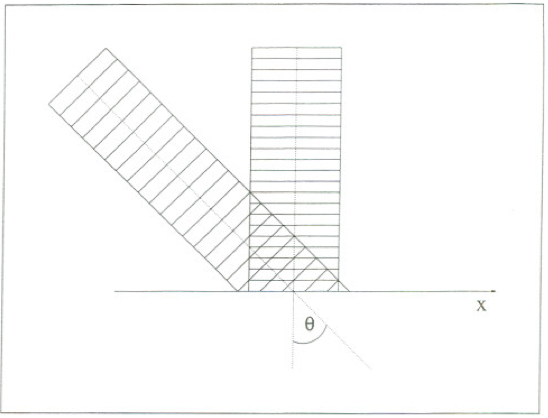
\includegraphics[width = \textwidth]{BilderTheo/Intebeb.png}
\caption{Interferenz zweier ebener Wellen\protect\footnotemark[1]}
\end{minipage}
\begin{minipage}{0.49\textwidth}
\centering 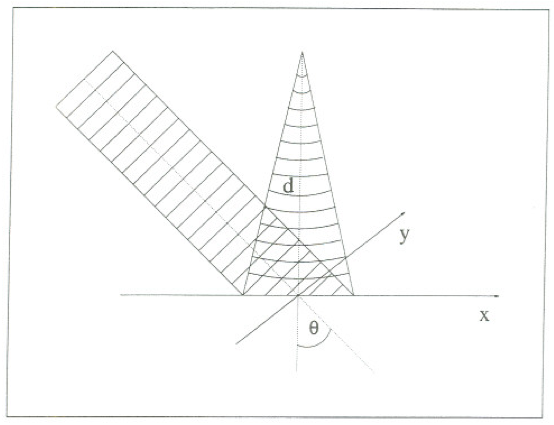
\includegraphics[width = \textwidth]{BilderTheo/Intebkug.png}
\caption{Interferenz einer ebenen Welle mit einer Kugelwelle\protect\footnotemark[1]}
\end{minipage}
\end{figure}

Tritt Licht auf eine Öffnung oder an einen Rand, so wird es an diesem gebeugt. Dies heißt, dass die nach dem Huygensschen Prinzip\footnote[2]{Jeder Punkt einer Wellenfront kann als Ausgangspunkt einer neuen, kugelförmigen Welle betrachtet werden.} an dieser Oberfläche entstehenden Kugelwellen gegenseitig interferieren und als Resultat die Intensität der Welle an einem Punkt in der Raumzeit durch die resultierende Intensität aller Teilwellen gegeben ist. Bei den Intensitätsmaxima (konstruktive Interferenz), die z.B. auf einem Schirm betrachtet werden können, spricht man von Beugungsordnungen. Das Verhältnis der Intensität der ersten Ordnung zur einfallenden Intensität, nennt man den Beugungswirkungsgrad:

\begin{equation} \epsilon = \frac{I (1.Ordnung)}{I(einfallend)} \end{equation}

Die Beugung kann im allgemeinen mit dem sogenannten Beugungsintegral berechnet werden. Bei der mathematischen Berechnung der Beugung an einer Apertur unterscheidet man zwischen 2 Näherungen, nämlich der Fraunhofer- und der Fresnelnäherung. Die Fraunhofer-Näherung sieht die Apertur als sehr klein, und die Distanz des beobachteten Beugungsmusters von dieser als sehr groß an. Das Beugungsintegral wird in diesem Fall gerade die Fouriertransformierte der Apertur. Die Fresnel-Näherung geht von einer kleinen Distanz zwischen Apertur und Schirm aus, und somit müssen weitere Terme betrachtet werden. Das Beugungsintegral wird in diesem Fall komplizierter, da auch quadratische Terme einfließen.

\footnotetext[3]{Demtröder, Wolfgang: \emph{Experimentalphysik 2: Elektrizität und Optik}, Kaiserslautern, 2008}

\begin{figure}[H]
\centering 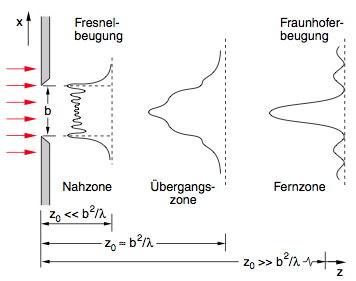
\includegraphics[width = 0.6\textwidth]{BilderTheo/FraunhoferFresnel.png}
\caption{Fraunhofer und Fresnelbeugung\protect\footnotemark[3]}
\end{figure}

\subsubsection{Kohärenz und Kohärenzlänge}

Zwei Wellen sind kohärent, wenn sie die gleiche Frequenz und eine konstante Phasendifferenz haben. Ihre Interferenz ist somit stationär und ortsfest, was in vielen Experimenten von großem Nutzen ist. Nur Wellen, die von einem gleichen Emissionsprozess stammen können kohärent sein. Die Kohärenz zweier Strahlen ist jedoch begrenzt durch ihren Weglängenunterschied. Ist dieser größer als die sogenannte Kohärenzlänge, so ist das Interferenzmuster nicht mehr stationär, d.h. die Strahlen werden inkohärent. 

%Michelson-Interferometer, Beugung am Amplituden/Phasengitter





















